%%%%%%%%%%%%%%%%%%%%%%%%%%%%%%%%%%%%%%%%%%%%%%%%%%%%%%%%%%%%%%%%%%%%%%%%%%%%%%%%%%%%%%%%%%%%%%%%%%%%%%%%%%%%%%%%%%%%%%%%%%%%%%%%%%%%%%%%%%%%%%%%%%%%%%%%%%%%%%%%%%%
% Written By Michael Brodskiy
% Class: Quantum Mechanics
% Professor: G. Fiete
%%%%%%%%%%%%%%%%%%%%%%%%%%%%%%%%%%%%%%%%%%%%%%%%%%%%%%%%%%%%%%%%%%%%%%%%%%%%%%%%%%%%%%%%%%%%%%%%%%%%%%%%%%%%%%%%%%%%%%%%%%%%%%%%%%%%%%%%%%%%%%%%%%%%%%%%%%%%%%%%%%%

\include{Includes.tex}

\title{Lecture 1}
\date{\today}
\author{Michael Brodskiy\\ \small Professor: G. Fiete}

\begin{document}

\maketitle

\begin{itemize}

  \item Key Features of Quantum Mechanics

    \begin{enumerate}

      \item Probabilistic outcome of measurements

        \begin{itemize}

          \item Compute probabilities \underline{exactly}, and that is the most complete information possible

        \end{itemize}

      \item Dual wave-particle nature of mature

        \begin{itemize}

          \item Which one we observe depends on the experiment performed

        \end{itemize}

      \item Conjugate variables (from classical mechanics) develop ``uncertainty'' relations

        \begin{itemize}

          \item Wave theory relation:

            $$\Delta x\Delta p\geq \hbar$$
            $$\Delta E \Delta t\geq \hbar$$

          \item Classical mechanics is ``contained'' in Quantum mechanics, which includes classical electricity and magnetism

        \end{itemize}

      \item Every particle and object built from particles, including light, falls into one of two classes:

        \begin{itemize}

          \item Fermions (spin is any odd multiple of $\hbar/2$)

            \begin{itemize}
                
              \item Electrons are an example

            \end{itemize}

          \item Bosons (spin is an integer multiple of $\hbar$, including 0)

            \begin{itemize}

              \item Photons are an example

            \end{itemize}

        \end{itemize}

      \item The properties of Quantum mechanics not falling into features 1-4 are largely familiar from classical physics

    \end{enumerate}

  \item Similar but Different

    \begin{itemize}

      \item Every electron has \underline{exactly} the same spin, charge, and mass

      \item Every photon has \underline{exactly} the same spin, charge, and mass

      \item This indicates no inequality among particles of the same type

    \end{itemize}

  \item Time-Evolution in Quantum Mechanics

    \begin{itemize}

      \item Time-evolution is given by the Hamiltonian, $\mathcal{H}$

      \item Hamilton's Equations give us:

        $$\frac{d\vec{q}}{dt}=\frac{\partial \mathcal{H}}{\partial \vec{p}}$$

      \item We may write the Hamiltonian as:

        $$\mathcal{H}=\frac{\vec{p}^2}{2m}\longrightarrow \frac{\partial \mathcal{H}}{\partial \vec{p}}=\frac{\vec{p}}{m}=\vec{v}$$

      \item Alternatively, we may write the force as:

        $$\vec{F}=\frac{d\vec{p}}{dt}=-\frac{\partial \mathcal{H}}{\partial\vec{q}}$$

    \end{itemize}

  \item Stern-Gerlach Experiments

    \begin{itemize}
        
      \item Took place in 1922 with Otto Stern and Walther Gerlach

      \item The act of observing a quantum particle affects its measurable properties in a way foreign to our experience

      \item The experiment looks like this:

        \begin{figure}[H]
          \centering
          \tikzset{every picture/.style={line width=0.75pt}} %set default line width to 0.75pt        

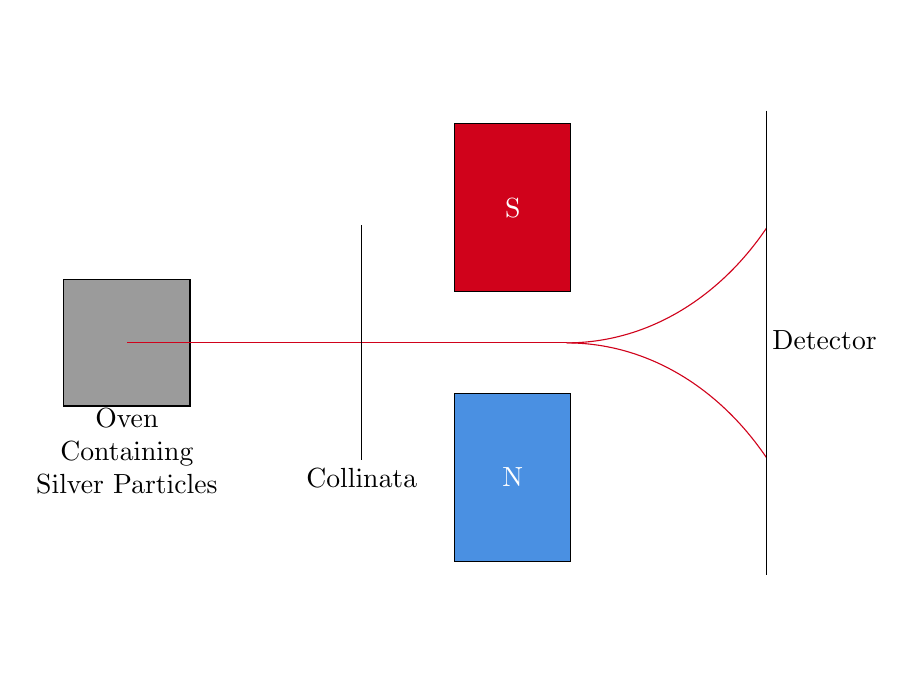
\begin{tikzpicture}[x=0.75pt,y=0.75pt,yscale=-.8,xscale=.8]
%uncomment if require: \path (0,375); %set diagram left start at 0, and has height of 375

%Shape: Square [id:dp14421103605944618] 
\draw  [fill={rgb, 255:red, 155; green, 155; blue, 155 }  ,fill opacity=1 ] (100,128) -- (176,128) -- (176,204) -- (100,204) -- cycle ;
%Straight Lines [id:da6727148484422872] 
\draw [color={rgb, 255:red, 208; green, 2; blue, 27 }  ,draw opacity=1 ]   (279.42,166) -- (138,166) ;
%Straight Lines [id:da8380240359625067] 
\draw    (279.42,95.29) -- (279.42,236.71) ;
%Shape: Rectangle [id:dp32874348023480093] 
\draw  [fill={rgb, 255:red, 208; green, 2; blue, 27 }  ,fill opacity=1 ] (335.42,34) -- (405.42,34) -- (405.42,135.29) -- (335.42,135.29) -- cycle ;
%Shape: Rectangle [id:dp31052784363324215] 
\draw  [fill={rgb, 255:red, 74; green, 144; blue, 226 }  ,fill opacity=1 ] (335.42,196.29) -- (405.42,196.29) -- (405.42,297.58) -- (335.42,297.58) -- cycle ;
%Straight Lines [id:da09102819630459058] 
\draw [color={rgb, 255:red, 208; green, 2; blue, 27 }  ,draw opacity=1 ]   (402.84,166) -- (279.42,166) ;
%Shape: Arc [id:dp14380617240917248] 
\draw  [draw opacity=0] (402.84,166) .. controls (402.84,166) and (402.84,166) .. (402.84,166) .. controls (451.32,166) and (494.63,192.92) .. (523.21,235.14) -- (402.84,355.5) -- cycle ; \draw  [color={rgb, 255:red, 208; green, 2; blue, 27 }  ,draw opacity=1 ] (402.84,166) .. controls (402.84,166) and (402.84,166) .. (402.84,166) .. controls (451.32,166) and (494.63,192.92) .. (523.21,235.14) ;  
%Shape: Arc [id:dp018293912875773533] 
\draw  [draw opacity=0] (402.84,166) .. controls (402.84,166) and (402.84,166) .. (402.84,166) .. controls (451.32,166) and (494.63,139.08) .. (523.21,96.86) -- (402.84,-23.5) -- cycle ; \draw  [color={rgb, 255:red, 208; green, 2; blue, 27 }  ,draw opacity=1 ] (402.84,166) .. controls (402.84,166) and (402.84,166) .. (402.84,166) .. controls (451.32,166) and (494.63,139.08) .. (523.21,96.86) ;  
%Straight Lines [id:da21129461638831382] 
\draw    (523.21,164.43) -- (523.21,305.85) ;
%Straight Lines [id:da4601124961028422] 
\draw    (523.21,26.15) -- (523.21,167.57) ;

% Text Node
\draw (138,204) node [anchor=north] [inner sep=0.75pt]   [align=left] {\begin{minipage}[lt]{70.19pt}\setlength\topsep{0pt}
\begin{center}
Oven \\Containing \\Silver Particles
\end{center}

\end{minipage}};
% Text Node
\draw (279.42,239.71) node [anchor=north] [inner sep=0.75pt]   [align=left] {\begin{minipage}[lt]{42.43pt}\setlength\topsep{0pt}
\begin{center}
Collinata
\end{center}

\end{minipage}};
% Text Node
\draw (370.42,84.64) node  [color={rgb, 255:red, 255; green, 255; blue, 255 }  ,opacity=1 ] [align=left] {S};
% Text Node
\draw (370.42,246.93) node  [color={rgb, 255:red, 255; green, 255; blue, 255 }  ,opacity=1 ] [align=left] {N};
% Text Node
\draw (525.21,164.43) node [anchor=west] [inner sep=0.75pt]   [align=left] {Detector};


\end{tikzpicture}

          \caption{Set Up of Stern-Gerlach Experiment}
          \label{fig:1}
        \end{figure}

      \item Assuming an atom has a monopole moment, $\vec{\mu}$, the potential energy of the interaction with a magnetic field $\vec{B}$ is $E=\vec{\mu}\vec{B}$

      \item Consider a classical description of the atom's moment:

        $$\mu=IA$$

        \begin{itemize}

          \item Where $I$ is the electrical current and $A$ is the area of the loop

        \end{itemize}

      \item A particle of charge $q$ traveling at speed $v$ in a circle of radius $r$ gives us:

        $$\mu=\frac{qvr}{2}=\frac{qL}{2m}$$

        \begin{itemize}

          \item Where $L=mvr$ is the orbitable angular momentum

        \end{itemize}

      \item Particles carry an intrinsic angular momentum, $\vec{S}$, called spin

        $$\vec{\mu}=\frac{gq\vec{S}}{2m}$$

        \begin{itemize}

          \item Where $g$ is the gyroscopic ratio

        \end{itemize}

      \item Noting that silver atoms were used is important, as different atoms give different results. Considering the shell filling of silver, we know that it extends to a singular atom in the $5s$ shell.

        \begin{itemize}

          \item Since the mass of the nucleus $\geq 2000m_e$, we find a ratio of magnetic moments as:

            $$\frac{\vec{\mu}_{nuc}}{\vec{\mu}_{e^-}}<<1$$

          \item Hence, we have $\vec{\mu}_{\text{Ag}}=-g\dfrac{e}{2m_e}\vec{S}$, where $e$ is the magnitude of an electron's charge

          \item This produces a force of $F_z=-g\dfrac{e}{2m_e}S_z\cdot\dfrac{2B_z}{2z}$

          \item Thus, the deflection of the beam in the Stern-Gerlach experiment is a measure of the projection of the intrinsic spin onto the $z$-axis

          \item Note, the heat of the oven randomizes the direction of $\vec{\mu}$, and, classicly, we have $S_z=|\vec{S}|\cos(\theta)$ and should be continuous over an $S_z$ range given by: $-|\vec{S}|\leq S_z\leq |\vec{S}|$

            \begin{itemize}

              \item But, only two beams are observed!

                \begin{itemize}

                  \item Only two $S_z$ components are possible, since $S_z=\pm \hbar/2$

                \end{itemize}

            \end{itemize}

        \end{itemize}

      \item We know:

        $$\hbar\approx=1.0546\cdot10^{-34}[\si{\joule\second}]=6.5821\cdot10^{-16}[\si{eV\second}]$$

        $$\hbar=\frac{h}{2\pi}\text{ (Planck's Constant)}$$

        \begin{itemize}

          \item This indicates a quantization of an electron's intrinsic angular momentum along the $z$ axis

          \item In the case that $S_z=+\hbar/2$, we call this spin ``up''

          \item In the case that $S_z=-\hbar/2$, we call this spin ``down''

          \item The quantity $S_z$ itself is called an ``observable''

          \item The device depicted within the Stern-Gerlach experiment is called an ``analyzer'', since it sorts the input into two possible outputs

          \item New notation: $S_z=+\hbar/2$ can be written in Dirac notation as:

            $$\ket{+\frac{\hbar}{2}}\Longrightarrow \ket{+}$$

          \item The negative (down) spin becomes:

            $$\ket{-\frac{\hbar}{2}}\Longrightarrow \ket{-}$$

          \item A ``ket'' can be depicted as follows:

            $$\ket{\cdot}$$

            \begin{itemize}

              \item Or, in its general form:

            $$\ket{\psi}$$

            \end{itemize}

          \item Note that for up and down spin, occasionally one may encounter:

            $$\ket{+}=\ket{\uparrow}$$
            $$\ket{-}=\ket{\downarrow}$$

        \end{itemize}

      \item Experiment 1:

        \begin{figure}[H]
          \centering
          \tikzset{every picture/.style={line width=0.75pt}} %set default line width to 0.75pt        

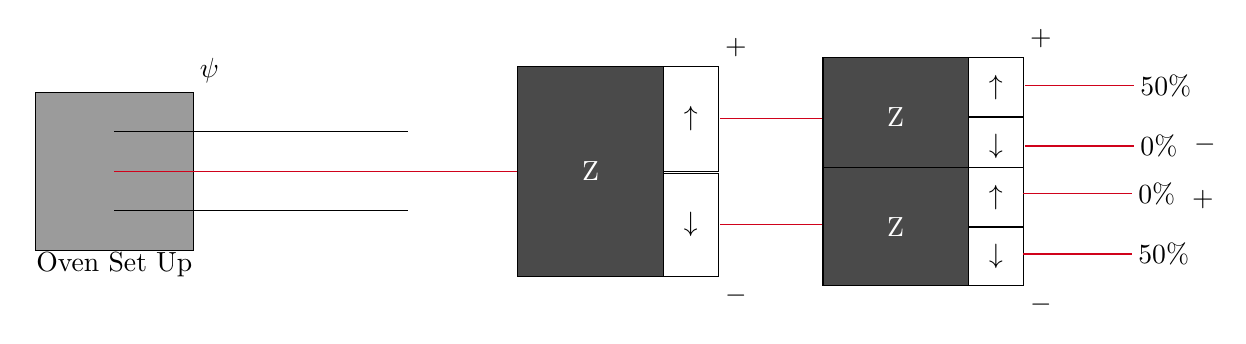
\begin{tikzpicture}[x=0.75pt,y=0.75pt,yscale=-1,xscale=1]
%uncomment if require: \path (0,375); %set diagram left start at 0, and has height of 375

%Shape: Square [id:dp14421103605944618] 
\draw  [fill={rgb, 255:red, 155; green, 155; blue, 155 }  ,fill opacity=1 ] (64,128) -- (140,128) -- (140,204) -- (64,204) -- cycle ;
%Straight Lines [id:da6727148484422872] 
\draw [color={rgb, 255:red, 208; green, 2; blue, 27 }  ,draw opacity=1 ]   (243.42,166) -- (102,166) ;
%Shape: Rectangle [id:dp31052784363324215] 
\draw  [fill={rgb, 255:red, 74; green, 74; blue, 74 }  ,fill opacity=1 ] (296.42,115.36) -- (366.42,115.36) -- (366.42,216.64) -- (296.42,216.64) -- cycle ;
%Straight Lines [id:da9714115391207371] 
\draw    (243.42,147) -- (102,147) ;
%Straight Lines [id:da9565511475124852] 
\draw    (243.42,185) -- (102,185) ;
%Straight Lines [id:da5775689584288694] 
\draw [color={rgb, 255:red, 208; green, 2; blue, 27 }  ,draw opacity=1 ]   (295.84,166) -- (243.42,166) ;
%Shape: Rectangle [id:dp34780699384586333] 
\draw  [fill={rgb, 255:red, 255; green, 255; blue, 255 }  ,fill opacity=1 ] (366.42,167) -- (393,167) -- (393,216.64) -- (366.42,216.64) -- cycle ;
%Shape: Rectangle [id:dp9674012952324293] 
\draw  [fill={rgb, 255:red, 255; green, 255; blue, 255 }  ,fill opacity=1 ] (366.42,115.36) -- (393,115.36) -- (393,166) -- (366.42,166) -- cycle ;
%Straight Lines [id:da8039050506004896] 
\draw [color={rgb, 255:red, 208; green, 2; blue, 27 }  ,draw opacity=1 ]   (446.13,140.68) -- (393.71,140.68) ;
%Straight Lines [id:da5371523365899473] 
\draw [color={rgb, 255:red, 208; green, 2; blue, 27 }  ,draw opacity=1 ]   (446.13,191.82) -- (393.71,191.82) ;
%Shape: Rectangle [id:dp5066877735662358] 
\draw  [fill={rgb, 255:red, 74; green, 74; blue, 74 }  ,fill opacity=1 ] (443.42,111.36) -- (513.42,111.36) -- (513.42,168) -- (443.42,168) -- cycle ;
%Shape: Rectangle [id:dp7068517018359358] 
\draw  [fill={rgb, 255:red, 255; green, 255; blue, 255 }  ,fill opacity=1 ] (513.42,140.24) -- (540,140.24) -- (540,168) -- (513.42,168) -- cycle ;
%Shape: Rectangle [id:dp5547396655118183] 
\draw  [fill={rgb, 255:red, 255; green, 255; blue, 255 }  ,fill opacity=1 ] (513.42,111.36) -- (540,111.36) -- (540,139.68) -- (513.42,139.68) -- cycle ;

%Straight Lines [id:da925156022518015] 
\draw [color={rgb, 255:red, 208; green, 2; blue, 27 }  ,draw opacity=1 ]   (593.13,124.68) -- (540.71,124.68) ;
%Straight Lines [id:da995628624290608] 
\draw [color={rgb, 255:red, 208; green, 2; blue, 27 }  ,draw opacity=1 ]   (593.13,153.82) -- (540.71,153.82) ;
%Shape: Rectangle [id:dp6769071252491495] 
\draw  [fill={rgb, 255:red, 74; green, 74; blue, 74 }  ,fill opacity=1 ] (443.42,164.36) -- (513.42,164.36) -- (513.42,221) -- (443.42,221) -- cycle ;
%Shape: Rectangle [id:dp6306771616992262] 
\draw  [fill={rgb, 255:red, 255; green, 255; blue, 255 }  ,fill opacity=1 ] (513.42,193.24) -- (540,193.24) -- (540,221) -- (513.42,221) -- cycle ;
%Shape: Rectangle [id:dp43240360470130335] 
\draw  [fill={rgb, 255:red, 255; green, 255; blue, 255 }  ,fill opacity=1 ] (513.42,164.36) -- (540,164.36) -- (540,192.68) -- (513.42,192.68) -- cycle ;

%Straight Lines [id:da3774129227180918] 
\draw [color={rgb, 255:red, 208; green, 2; blue, 27 }  ,draw opacity=1 ]   (592.13,176.68) -- (539.71,176.68) ;
%Straight Lines [id:da9566074019333357] 
\draw [color={rgb, 255:red, 208; green, 2; blue, 27 }  ,draw opacity=1 ]   (592.13,205.82) -- (539.71,205.82) ;

% Text Node
\draw (102,204) node [anchor=north] [inner sep=0.75pt]   [align=left] {\begin{minipage}[lt]{61.13pt}\setlength\topsep{0pt}
\begin{center}
Oven Set Up
\end{center}

\end{minipage}};
% Text Node
\draw (331.42,166) node  [color={rgb, 255:red, 255; green, 255; blue, 255 }  ,opacity=1 ] [align=left] {Z};
% Text Node
\draw (379.71,140.68) node    {$\uparrow $};
% Text Node
\draw (379.71,191.82) node  [rotate=-180]  {$\uparrow $};
% Text Node
\draw (142,124.6) node [anchor=south west] [inner sep=0.75pt]    {$\ket{\psi }$};
% Text Node
\draw (395,111.96) node [anchor=south west] [inner sep=0.75pt]    {$\ket{+}$};
% Text Node
\draw (395,220.04) node [anchor=north west][inner sep=0.75pt]    {$\ket{-}$};
% Text Node
\draw (542,107.96) node [anchor=south west] [inner sep=0.75pt]    {$\ket{+}$};
% Text Node
\draw (542,224.4) node [anchor=north west][inner sep=0.75pt]    {$\ket{-}$};
% Text Node
\draw (478.42,139.68) node  [color={rgb, 255:red, 255; green, 255; blue, 255 }  ,opacity=1 ] [align=left] {Z};
% Text Node
\draw (526.71,125.52) node    {$\uparrow $};
% Text Node
\draw (526.71,154.12) node  [rotate=-180]  {$\uparrow $};
% Text Node
\draw (595.13,124.68) node [anchor=west] [inner sep=0.75pt]    {$50\%$};
% Text Node
\draw (595.13,153.82) node [anchor=west] [inner sep=0.75pt]    {$0\%$};
% Text Node
\draw (526.71,207.12) node  [rotate=-180]  {$\uparrow $};
% Text Node
\draw (526.71,178.52) node    {$\uparrow $};
% Text Node
\draw (478.42,192.68) node  [color={rgb, 255:red, 255; green, 255; blue, 255 }  ,opacity=1 ] [align=left] {Z};
% Text Node
\draw (594.13,176.68) node [anchor=west] [inner sep=0.75pt]    {$0\%$};
% Text Node
\draw (594.13,205.82) node [anchor=west] [inner sep=0.75pt]    {$50\%$};
% Text Node
\draw (620,185.28) node [anchor=south west] [inner sep=0.75pt]    {$\ket{+}$};
% Text Node
\draw (621,147.4) node [anchor=north west][inner sep=0.75pt]    {$\ket{-}$};


\end{tikzpicture}

          \caption{Experimental Setup}
          \label{fig:2}
        \end{figure}

        \begin{itemize}

          \item Although both Stern-Gerlach analyzers in the experiment are the same, they play different roles

            \begin{itemize}

              \item The first analyzer prepares the beam and the second analyzer measures the beam

              \item The first analyzer is often referred to as a state preparation device

            \end{itemize}

        \end{itemize}

      \item Experiment 2:

        \begin{figure}[H]
          \centering
          \tikzset{every picture/.style={line width=0.75pt}} %set default line width to 0.75pt        

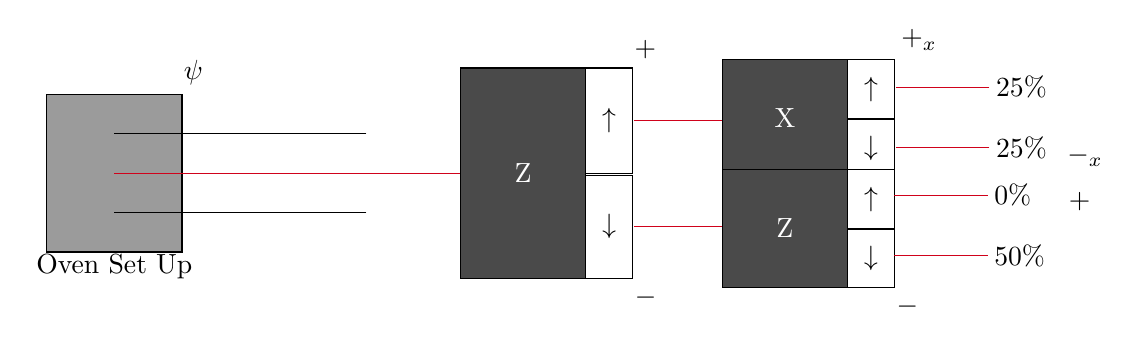
\begin{tikzpicture}[x=0.75pt,y=0.75pt,yscale=-1,xscale=1]
%uncomment if require: \path (0,375); %set diagram left start at 0, and has height of 375

%Shape: Rectangle [id:dp14421103605944618] 
\draw  [fill={rgb, 255:red, 155; green, 155; blue, 155 }  ,fill opacity=1 ] (13.01,128) -- (78.24,128) -- (78.24,204) -- (13.01,204) -- cycle ;
%Straight Lines [id:da6727148484422872] 
\draw [color={rgb, 255:red, 208; green, 2; blue, 27 }  ,draw opacity=1 ]   (167.01,166) -- (45.63,166) ;
%Shape: Rectangle [id:dp31052784363324215] 
\draw  [fill={rgb, 255:red, 74; green, 74; blue, 74 }  ,fill opacity=1 ] (212.51,115.36) -- (272.59,115.36) -- (272.59,216.64) -- (212.51,216.64) -- cycle ;
%Straight Lines [id:da9714115391207371] 
\draw    (167.01,147) -- (45.63,147) ;
%Straight Lines [id:da9565511475124852] 
\draw    (167.01,185) -- (45.63,185) ;
%Straight Lines [id:da5775689584288694] 
\draw [color={rgb, 255:red, 208; green, 2; blue, 27 }  ,draw opacity=1 ]   (212.01,166) -- (167.01,166) ;
%Shape: Rectangle [id:dp34780699384586333] 
\draw  [fill={rgb, 255:red, 255; green, 255; blue, 255 }  ,fill opacity=1 ] (272.59,167) -- (295.4,167) -- (295.4,216.64) -- (272.59,216.64) -- cycle ;
%Shape: Rectangle [id:dp9674012952324293] 
\draw  [fill={rgb, 255:red, 255; green, 255; blue, 255 }  ,fill opacity=1 ] (272.59,115.36) -- (295.4,115.36) -- (295.4,166) -- (272.59,166) -- cycle ;
%Straight Lines [id:da8039050506004896] 
\draw [color={rgb, 255:red, 208; green, 2; blue, 27 }  ,draw opacity=1 ]   (341.01,140.68) -- (296.01,140.68) ;
%Straight Lines [id:da5371523365899473] 
\draw [color={rgb, 255:red, 208; green, 2; blue, 27 }  ,draw opacity=1 ]   (341.01,191.82) -- (296.01,191.82) ;
%Shape: Rectangle [id:dp5066877735662358] 
\draw  [fill={rgb, 255:red, 74; green, 74; blue, 74 }  ,fill opacity=1 ] (338.68,111.36) -- (398.77,111.36) -- (398.77,168) -- (338.68,168) -- cycle ;
%Shape: Rectangle [id:dp7068517018359358] 
\draw  [fill={rgb, 255:red, 255; green, 255; blue, 255 }  ,fill opacity=1 ] (398.77,140.24) -- (421.58,140.24) -- (421.58,168) -- (398.77,168) -- cycle ;
%Shape: Rectangle [id:dp5547396655118183] 
\draw  [fill={rgb, 255:red, 255; green, 255; blue, 255 }  ,fill opacity=1 ] (398.77,111.36) -- (421.58,111.36) -- (421.58,139.68) -- (398.77,139.68) -- cycle ;

%Straight Lines [id:da925156022518015] 
\draw [color={rgb, 255:red, 208; green, 2; blue, 27 }  ,draw opacity=1 ]   (467.19,124.68) -- (422.19,124.68) ;
%Straight Lines [id:da995628624290608] 
\draw [color={rgb, 255:red, 208; green, 2; blue, 27 }  ,draw opacity=1 ]   (467.19,153.82) -- (422.19,153.82) ;
%Shape: Rectangle [id:dp6769071252491495] 
\draw  [fill={rgb, 255:red, 74; green, 74; blue, 74 }  ,fill opacity=1 ] (338.68,164.36) -- (398.77,164.36) -- (398.77,221) -- (338.68,221) -- cycle ;
%Shape: Rectangle [id:dp6306771616992262] 
\draw  [fill={rgb, 255:red, 255; green, 255; blue, 255 }  ,fill opacity=1 ] (398.77,193.24) -- (421.58,193.24) -- (421.58,221) -- (398.77,221) -- cycle ;
%Shape: Rectangle [id:dp43240360470130335] 
\draw  [fill={rgb, 255:red, 255; green, 255; blue, 255 }  ,fill opacity=1 ] (398.77,164.36) -- (421.58,164.36) -- (421.58,192.68) -- (398.77,192.68) -- cycle ;

%Straight Lines [id:da3774129227180918] 
\draw [color={rgb, 255:red, 208; green, 2; blue, 27 }  ,draw opacity=1 ]   (466.33,176.68) -- (421.33,176.68) ;
%Straight Lines [id:da9566074019333357] 
\draw [color={rgb, 255:red, 208; green, 2; blue, 27 }  ,draw opacity=1 ]   (466.33,205.82) -- (421.33,205.82) ;

% Text Node
\draw (45.63,204) node [anchor=north] [inner sep=0.75pt]   [align=left] {\begin{minipage}[lt]{61.13pt}\setlength\topsep{0pt}
\begin{center}
Oven Set Up
\end{center}

\end{minipage}};
% Text Node
\draw (242.55,166) node  [color={rgb, 255:red, 255; green, 255; blue, 255 }  ,opacity=1 ] [align=left] {Z};
% Text Node
\draw (284,140.68) node    {$\uparrow $};
% Text Node
\draw (284,191.82) node  [rotate=-180]  {$\uparrow $};
% Text Node
\draw (77.91,124.6) node [anchor=south west] [inner sep=0.75pt]    {$\ket{\psi }$};
% Text Node
\draw (295.07,111.96) node [anchor=south west] [inner sep=0.75pt]    {$\ket{+}$};
% Text Node
\draw (295.14,220.04) node [anchor=north west][inner sep=0.75pt]    {$\ket{-}$};
% Text Node
\draw (423.58,107.96) node [anchor=south west] [inner sep=0.75pt]    {$\ket{+}_{x}$};
% Text Node
\draw (421.32,224.4) node [anchor=north west][inner sep=0.75pt]    {$\ket{-}$};
% Text Node
\draw (368.73,139.68) node  [color={rgb, 255:red, 255; green, 255; blue, 255 }  ,opacity=1 ] [align=left] {X};
% Text Node
\draw (410.17,125.52) node    {$\uparrow $};
% Text Node
\draw (410.17,154.12) node  [rotate=-180]  {$\uparrow $};
% Text Node
\draw (410.17,207.12) node  [rotate=-180]  {$\uparrow $};
% Text Node
\draw (410.17,178.52) node    {$\uparrow $};
% Text Node
\draw (368.73,192.68) node  [color={rgb, 255:red, 255; green, 255; blue, 255 }  ,opacity=1 ] [align=left] {Z};
% Text Node
\draw (468.33,176.68) node [anchor=west] [inner sep=0.75pt]    {$0\%$};
% Text Node
\draw (468.33,205.82) node [anchor=west] [inner sep=0.75pt]    {$50\%$};
% Text Node
\draw (504.2,185.28) node [anchor=south west] [inner sep=0.75pt]    {$\ket{+}$};
% Text Node
\draw (503.58,163.96) node [anchor=south west] [inner sep=0.75pt]    {$\ket{-}_{x}$};
% Text Node
\draw (469.19,124.68) node [anchor=west] [inner sep=0.75pt]    {$25\%$};
% Text Node
\draw (469.19,153.82) node [anchor=west] [inner sep=0.75pt]    {$25\%$};


\end{tikzpicture}

          \caption{Experimental Setup}
          \label{fig:3}
        \end{figure}

        \begin{itemize}

          \item The second analyzer is rotated by $90^{\circ}$ with respect to the first and aligned with the $x$-axis

            \begin{itemize}

              \item Only two possible outputs from second analyzer

              \item Results would be unchanged if we used the lower part of the first analyzer

              \item One can not predict which of the second analyzer parts any particular atom will emerge from

              \item These results highlight the probablistic nature of quantum mechanics; quantum mechanics is a complete description of reality (as far as we know)

            \end{itemize}

        \end{itemize}

      \item Experiment 3:

        \begin{figure}[H]
          \centering
          \include{Figures/Stern-Gerlach4}
          \caption{Experimental Setup}
          \label{fig:4}
        \end{figure}
    
        \begin{itemize}

          \item This tells us that the $S_x$ and $S_z$ are incompatible observables, which means we can not know the values of both simultaneously

        \end{itemize}

      \item Experiment 4:

        \begin{figure}[H]
          \centering
          \include{Figures/Stern-Gerlach5a}
          \caption{Experimental Setup Part One}
          \label{fig:5}
        \end{figure}

        \begin{figure}[H]
          \centering
          \tikzset{every picture/.style={line width=0.75pt}} %set default line width to 0.75pt        

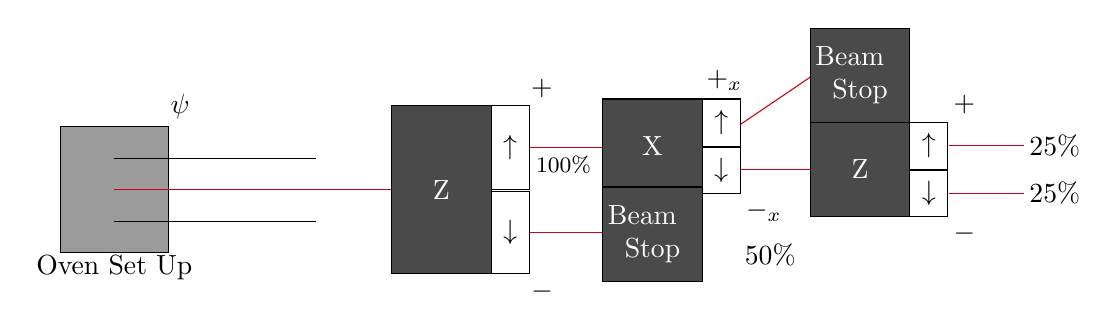
\begin{tikzpicture}[x=0.75pt,y=0.75pt,yscale=-.8,xscale=.8]
%uncomment if require: \path (0,375); %set diagram left start at 0, and has height of 375

%Shape: Rectangle [id:dp14421103605944618] 
\draw  [fill={rgb, 255:red, 155; green, 155; blue, 155 }  ,fill opacity=1 ] (13.01,128) -- (78.24,128) -- (78.24,204) -- (13.01,204) -- cycle ;
%Straight Lines [id:da6727148484422872] 
\draw [color={rgb, 255:red, 208; green, 2; blue, 27 }  ,draw opacity=1 ]   (167.01,166) -- (45.63,166) ;
%Shape: Rectangle [id:dp31052784363324215] 
\draw  [fill={rgb, 255:red, 74; green, 74; blue, 74 }  ,fill opacity=1 ] (212.51,115.36) -- (272.59,115.36) -- (272.59,216.64) -- (212.51,216.64) -- cycle ;
%Straight Lines [id:da9714115391207371] 
\draw    (167.01,147) -- (45.63,147) ;
%Straight Lines [id:da9565511475124852] 
\draw    (167.01,185) -- (45.63,185) ;
%Straight Lines [id:da5775689584288694] 
\draw [color={rgb, 255:red, 208; green, 2; blue, 27 }  ,draw opacity=1 ]   (212.01,166) -- (167.01,166) ;
%Shape: Rectangle [id:dp34780699384586333] 
\draw  [fill={rgb, 255:red, 255; green, 255; blue, 255 }  ,fill opacity=1 ] (272.59,167) -- (295.4,167) -- (295.4,216.64) -- (272.59,216.64) -- cycle ;
%Shape: Rectangle [id:dp9674012952324293] 
\draw  [fill={rgb, 255:red, 255; green, 255; blue, 255 }  ,fill opacity=1 ] (272.59,115.36) -- (295.4,115.36) -- (295.4,166) -- (272.59,166) -- cycle ;
%Straight Lines [id:da8039050506004896] 
\draw [color={rgb, 255:red, 208; green, 2; blue, 27 }  ,draw opacity=1 ]   (341.01,140.68) -- (296.01,140.68) ;
%Straight Lines [id:da5371523365899473] 
\draw [color={rgb, 255:red, 208; green, 2; blue, 27 }  ,draw opacity=1 ]   (341.01,191.82) -- (296.01,191.82) ;
%Shape: Rectangle [id:dp5066877735662358] 
\draw  [fill={rgb, 255:red, 74; green, 74; blue, 74 }  ,fill opacity=1 ] (339.68,111.36) -- (399.77,111.36) -- (399.77,168) -- (339.68,168) -- cycle ;
%Shape: Rectangle [id:dp7068517018359358] 
\draw  [fill={rgb, 255:red, 255; green, 255; blue, 255 }  ,fill opacity=1 ] (399.77,140.24) -- (422.58,140.24) -- (422.58,168) -- (399.77,168) -- cycle ;
%Shape: Rectangle [id:dp5547396655118183] 
\draw  [fill={rgb, 255:red, 255; green, 255; blue, 255 }  ,fill opacity=1 ] (399.77,111.36) -- (422.58,111.36) -- (422.58,139.68) -- (399.77,139.68) -- cycle ;

%Straight Lines [id:da925156022518015] 
\draw [color={rgb, 255:red, 208; green, 2; blue, 27 }  ,draw opacity=1 ]   (465,98) -- (422.78,126.59) ;
%Straight Lines [id:da995628624290608] 
\draw [color={rgb, 255:red, 208; green, 2; blue, 27 }  ,draw opacity=1 ]   (468.19,153.82) -- (423.19,153.82) ;
%Shape: Rectangle [id:dp5083037352636465] 
\draw  [fill={rgb, 255:red, 74; green, 74; blue, 74 }  ,fill opacity=1 ] (339.68,164.36) -- (399.77,164.36) -- (399.77,221) -- (339.68,221) -- cycle ;
%Shape: Rectangle [id:dp3008323325045591] 
\draw  [fill={rgb, 255:red, 74; green, 74; blue, 74 }  ,fill opacity=1 ] (464.68,125.36) -- (524.77,125.36) -- (524.77,182) -- (464.68,182) -- cycle ;
%Shape: Rectangle [id:dp24796764616598033] 
\draw  [fill={rgb, 255:red, 255; green, 255; blue, 255 }  ,fill opacity=1 ] (524.77,154.24) -- (547.58,154.24) -- (547.58,182) -- (524.77,182) -- cycle ;
%Shape: Rectangle [id:dp4270203138981403] 
\draw  [fill={rgb, 255:red, 255; green, 255; blue, 255 }  ,fill opacity=1 ] (524.77,125.36) -- (547.58,125.36) -- (547.58,153.68) -- (524.77,153.68) -- cycle ;

%Straight Lines [id:da8067196861586373] 
\draw [color={rgb, 255:red, 208; green, 2; blue, 27 }  ,draw opacity=1 ]   (593.17,139.52) -- (548.17,139.52) ;
%Straight Lines [id:da7594531119094955] 
\draw [color={rgb, 255:red, 208; green, 2; blue, 27 }  ,draw opacity=1 ]   (593.17,168.12) -- (548.17,168.12) ;
%Shape: Rectangle [id:dp228315118501631] 
\draw  [fill={rgb, 255:red, 74; green, 74; blue, 74 }  ,fill opacity=1 ] (464.68,68.71) -- (524.77,68.71) -- (524.77,125.36) -- (464.68,125.36) -- cycle ;

% Text Node
\draw (45.63,204) node [anchor=north] [inner sep=0.75pt]   [align=left] {\begin{minipage}[lt]{61.13pt}\setlength\topsep{0pt}
\begin{center}
Oven Set Up
\end{center}

\end{minipage}};
% Text Node
\draw (242.55,166) node  [color={rgb, 255:red, 255; green, 255; blue, 255 }  ,opacity=1 ] [align=left] {Z};
% Text Node
\draw (284,140.68) node    {$\uparrow $};
% Text Node
\draw (284,191.82) node  [rotate=-180]  {$\uparrow $};
% Text Node
\draw (77.91,124.6) node [anchor=south west] [inner sep=0.75pt]    {$\ket{\psi }$};
% Text Node
\draw (295.07,111.96) node [anchor=south west] [inner sep=0.75pt]    {$\ket{+}$};
% Text Node
\draw (295.14,220.04) node [anchor=north west][inner sep=0.75pt]    {$\ket{-}$};
% Text Node
\draw (400.77,107.96) node [anchor=south west] [inner sep=0.75pt]    {$\ket{+}_{x}$};
% Text Node
\draw (369.73,139.68) node  [color={rgb, 255:red, 255; green, 255; blue, 255 }  ,opacity=1 ] [align=left] {X};
% Text Node
\draw (411.17,125.52) node    {$\uparrow $};
% Text Node
\draw (411.17,154.12) node  [rotate=-180]  {$\uparrow $};
% Text Node
\draw (595.17,139.52) node [anchor=west] [inner sep=0.75pt]    {$25\%$};
% Text Node
\draw (536.17,168.12) node  [rotate=-180]  {$\uparrow $};
% Text Node
\draw (536.17,139.52) node    {$\uparrow $};
% Text Node
\draw (494.73,153.68) node  [color={rgb, 255:red, 255; green, 255; blue, 255 }  ,opacity=1 ] [align=left] {Z};
% Text Node
\draw (595.17,168.12) node [anchor=west] [inner sep=0.75pt]    {$25\%$};
% Text Node
\draw (549.58,121.96) node [anchor=south west] [inner sep=0.75pt]    {$\ket{+}$};
% Text Node
\draw (549.58,185.4) node [anchor=north west][inner sep=0.75pt]    {$\ket{-}$};
% Text Node
\draw (369.73,192.68) node  [color={rgb, 255:red, 255; green, 255; blue, 255 }  ,opacity=1 ] [align=left] {\begin{minipage}[lt]{32.21pt}\setlength\topsep{0pt}
Beam 
\begin{center}
Stop
\end{center}

\end{minipage}};
% Text Node
\draw (298.01,144.08) node [anchor=north west][inner sep=0.75pt]    {\footnotesize $100\%$};
% Text Node
\draw (494.73,97.03) node  [color={rgb, 255:red, 255; green, 255; blue, 255 }  ,opacity=1 ] [align=left] {\begin{minipage}[lt]{32.21pt}\setlength\topsep{0pt}
Beam 
\begin{center}
Stop
\end{center}

\end{minipage}};
% Text Node
\draw (424.58,171.4) node [anchor=north west][inner sep=0.75pt]    {$\ket{-}_{x}$};
% Text Node
\draw (423.78,196.99) node [anchor=north west][inner sep=0.75pt]    {$50\%$};


\end{tikzpicture}

          \caption{Experimental Setup Part Two}
          \label{fig:6}
        \end{figure}

        \begin{figure}[H]
          \centering
          \include{Figures/Stern-Gerlach5c}
          \caption{Experimental Setup Part Three}
          \label{fig:7}
        \end{figure}

        \begin{itemize}

          \item Results are akin to the double slit experiment and destructive interference

        \end{itemize}

    \end{itemize}

  \item Quantum State Vectors

    \begin{itemize}

      \item The kets ($\ket{\psi}$) obey many rules of ordinary spacial vectors

      \item $\ket{\psi}$ is a quantum state vector and is part of a vector space called a Hilbert Space

      \item The dimensionality of the Hilbert Space is determined by the physics at hand

      \item In the Stern-Gerlach experiment the Hilbert Space has just two states ($\ket{+}$ and $\ket{-}$)

        \begin{itemize}

          \item These states form a basis like unit vectors $\hat{i},\hat{j},\hat{k}$ for 3-D space. These basis vectors are normalized, orthogonal, and complete
            
            \begin{itemize}

              \item Normailization: $\hat{i}\cdot\hat{i}=\hat{j}\cdot\hat{j}=\hat{k}\cdot\hat{k}=1$

              \item Orthogonality: $\hat{i}\cdot\hat{j}=\hat{i}\cdot\hat{k}=\hat{j}\cdot\hat{k}=0$

              \item Completeness: $\vec{A}=a_x\hat{i}+a_y\hat{j}+a_z\hat{k}$

              \item Note: The dot product (or scalar product) displayed in the normalization and orthogonality conditions is central to these properties

            \end{itemize}

          \item For the $S_z$ measurement, the basis states are: $\ket{+}$ and $\ket{-}$ and are referred to as the ``$S_z$ basis''

            \begin{itemize}

              \item Since this is a complete basis, a general state is (where $a$ and $b$ are complex numbers):

                $$\ket{\psi}=a\ket{+}+b\ket{-}$$

            \end{itemize}

          \item To discuss orthogonality and normalization (orthonormality) we need to understand how scalar products apply to kets

          \item The complex-conjugated quantum state vector is called a 'bra' in the Dirac notation of quantum mechanics (note the asterisk indicates the complex conjugate):

            $$\bra{\psi}=a^*\bra{+}+b^*\bra{-}$$

        \end{itemize}

      \item The scalar product in quantum mechanics is defined as:

        $$(\bra{\psi})(\ket{\psi})=\braket{\psi}$$

        \begin{itemize}

          \item ``bra-ket'' or bracket

          \item For example:

            $$(\bra{+})(\ket{-})=\bra{+}\ket{-}$$

          \item This defines an inner product between two state vectors

          \item In analogy to 3-D spatial vectors, this is also called a projection

          \item Given the analogs, we may write that normality is defined as:

            $$\braket{+}=\braket{-}=1$$

          \item Furthermore, orthogonality may be defined as:

            $$\bra{+}\ket{-}=\bra{-}\ket{+}=0$$

          \item Completeness is then defined as:

            $$\ket{\psi}=a\ket{+}+b\ket{-}$$

          \item With these components, we can then write:

            $$\bra{+}\ket{\psi}=\bra{+}(a\ket{+}+b\ket{-})=\bra{+|a}\ket{+}+\bra{+|b}\ket{-}=a\braket{+}+b\bra{+}\ket{-}$$

            \begin{itemize}

              \item This can then be simplified with our properties to get:

                $$\bra{+}\ket{\psi}=a$$

              \item Likewise, we may write:

                $$\bra{-}\ket{\psi}=b$$

            \end{itemize}

          \item Using these results, we may rewrite the wave function as:

            $$\ket{\psi}=\bra{+}\ket{\psi}\ket{+}+\bra{-}\ket{\psi}\ket{-}$$
            $$\ket{\psi}=\ket{+}\bra{+}\ket{\psi}+\ket{-}\bra{-}\ket{\psi}$$
            $$\ket{\psi}=\underbrace{(\ket{+}\bra{+}+\ket{-}\bra{-})}_1\ket{\psi}$$

            \begin{itemize}

              \item We can note that the identity is equivalent to one

            \end{itemize}

          \item We can also reverse the projection to write:

            $$\bra{\psi}\ket{+}=\bra{+|a^*}\ket{+}+\bra{-|b^*}\ket{+}=a^*\braket{+}+b^*\bra{-}\ket{+}=a^*$$

            \begin{itemize}

              \item This gives us the result that (note this holds for any state):

                $$\bra{\psi}\ket{+}=\bra{+}\ket{\psi}^*\Rightarrow \bra{\phi}\ket{\psi}=\bra{\psi}\ket{\phi}^*$$

              \item In quantum mechanics, state vectors must be normalized since they describe a situation where the quantum state has probability 1

                $$\braket{\psi}=(a^*\bra{+}+b^*\bra{-})(a\ket{+}+b\ket{-})$$
                $$=a^*a\braket{+}+a^*b\bra{+}\ket{-}+ab^*\bra{-}\ket{+}+b^*b\braket{-}$$
                $$\braket{\psi}=a^*a+b^*b=|a|^2+|b|^2=1$$

              \item Equivalently, we may write:

                $$|\bra{+}\ket{\psi}|^2+|\bra{-}\ket{\psi}|^2=1$$

            \end{itemize}

        \end{itemize}

      \item In quantum mechanics, the probability that the state $\ket{\psi}$ is measured as spin up is $P_{S_z=+\frac{\hbar}{2}}=|\bra{+}\ket{\psi}|^2$

      \item Equivalently, the probability that the state $\ket{\psi}$ is measures as spin down is $P_{S_z=-\frac{\hbar}{2}}=|\bra{-}\ket{\psi}|^2$

        \begin{itemize}

          \item We can use a shorthand notation of $P_+$ for $S_z=+\dfrac{\hbar}{2}$ and $P_-$ for $S_z=-\dfrac{\hbar}{2}$

          \item We may observe that the coefficients of the quantum state function contain the information regarding the probability

          \item This leads to Postulate 4 of Quantum Mechanics (for a 1/2-spin system)

            \begin{itemize}

              \item The probability of obtaining the value $\pm\hbar/2$ in a measurement of the observable, $S_z$, on a system in the state $\ket{\psi}$ is $P_{\pm}=|\bra{\pm}\ket{\psi}|^2$, where $\ket{\pm}$ is the basis ket of $S_z$ corresponding to the result $\pm\hbar/2$

              \item $\bra{-}\ket{\psi}$ is referred to as the probability amplitude (or just amplitude)

            \end{itemize}

        \end{itemize}

      \item For the Stern-Gerlach experiments in which a different axis was tested after the first analyzer, we may write:

        $$|_x\bra{+}\ket{+}|^2=|_x\bra{-}\ket{+}|^2=|_x\bra{+}\ket{-}|^2=|_x\bra{-}\ket{-}|^2=\frac{1}{2}$$

      \item Since $\ket{+}$ and $\ket{-}$ form a complete basis, we can write:

        $$\ket{+}_x=a\ket{+}+b\ket{-}$$
        $$\ket{-}_x=c\ket{+}+d\ket{-}$$

        \begin{itemize}

          \item Per the results of the Stern-Gerlach experiments, we may write:

            $$|a|^2=|b|^2=|c|^2=|d|^2=\frac{1}{2}$$

          \item This means:

            $$\ket{+}_x=\frac{1}{\sqrt{2}}\left( \ket{+}+e^{i\alpha}\ket{-} \right)$$
            $$\ket{-}_x=\frac{1}{\sqrt{2}}\left( \ket{+}+e^{-i\beta}\ket{-} \right)$$

          \item Therefore, only the relative phase of the weights are important

          \item If experiment 1 is repeated, but with both analyzers aligned in the $x$ direction, then one may find:

            $$P_{+x}=|\leftindex_x\braket{+}_x|^{2}=1$$
            $$P_{-x}=|\leftindex_x\bra{-}\ket{+}_x|^{2}=0$$

          \item Equivalently, we may write:

            $$\frac{1}{2}\left( 1+e^{i(\alpha-\beta)} \right)=0$$
            $$e^{i(\alpha-\beta)}=1$$

          \item And finally, we get our condition:

            $$e^{i\alpha}=e^{i\beta}$$

          \item We are free to choose $\alpha=\beta=0$

          \item Thus, we can express $x$-axis ket alignment as:

            $$\ket{\pm}_x=\frac{1}{\sqrt{2}}(\ket{+}\pm\ket{-})$$

        \end{itemize}

    \end{itemize}

  \item Superposition of States

    $$\ket{\psi}=a\ket{+}+b\ket{-}$$

    \begin{itemize}

      \item The above is a superposition state (or a coherent state) because of the importance of the relative phase of the two terms

      \item A contrasting state with different possible outcomes but no definite phase relation is called a mixed state
      
      \item A mixed state is not described by a quantum state $\ket{\psi}$, but instead a density matrix

      \item In matrix form, we can write:

        $$\ket{\pm}_x=\frac{1}{\sqrt{2}}\left( \begin{matrix} 1\\\pm1\end{matrix} \right)$$

        \begin{itemize}

          \item Note the top refers to the coefficient of the `up' $z$ state and the bottom refers to the coefficient of the `down' $z$ state. Given this, the basis states are:

            $$\ket{+}=\left( \begin{matrix} 1\\ 0\end{matrix} \right)\quad\text{ and }\quad\ket{-}=\left( \begin{matrix} 0\\ 1\end{matrix} \right)$$

          \item A general state may be written as:

            $$\ket{\psi}=\left( \begin{matrix} \bra{+}\ket{\psi}\\ \bra{-}\ket{\psi}\end{matrix} \right)$$

          \item For Hilbert Spaces whose dimensions are greater than 2, the matrix notation is generally more convenient

        \end{itemize}

      \item Repeating the earlier analysis but for the $y$ state, we get:

        $$\ket{\pm}_y=\frac{1}{\sqrt{2}}(\ket{+}\pm i\ket{-})$$

      \item In matrix notation this is equivalent to:

        $$\ket{\pm}_y=\left( \begin{matrix} 1\\ \pm i\end{matrix} \right)$$

    \end{itemize}

  \item General Quantum States

    \begin{itemize}

      \item Suppose we have an $N$-dimensional Hilbert Space with possible outcomes $\ket{a_1}$, $\ket{a_2}$,\ldots, $\ket{a_N}$

      \item We can then form the relation:

        $$\bra{a_i}\ket{a_j}=\delta_{ij}\quad\text{ orthonormality}$$

        \begin{itemize}

          \item With the Kroenecker Delta function being:

            $$\delta_{ij}=\left\{ \begin{array}{ll} 0,& i\neq j\\1,&i=j\end{array}$$

        \end{itemize}

      \item We can determine completeness using:

        $$\ket{\psi}=\sum_{i=1}^{N} (\bra{a_i}\ket{\psi})\ket{a_i}$$
        $$=\sum_{i=1}^{N} \ket{\psi}(\braket{a_i})$$
        $$=\ket{\psi}$$

          \begin{itemize}

            \item Here we see the identity matrix

          \end{itemize}

    \end{itemize}

  \item Postulates of Quantum Mechanics

    \begin{itemize}

      \item These can not be proven, but have been successfully tested in many experiments

    \end{itemize}

    \begin{enumerate}

      \item The state of a quantum system, including all of the information you can know about it, is represented by the $\ket{\psi}$

      \item A physical observable is represented mathematically by an operator $A$ that acts on kets

      \item The only possible result of a measurement of an observable is one of the eigenvalues of the corresponding operator $A$

      \item The probability of obtaining the eigenvalue $a_n$ in the measurement of the observable, $A$, on the system in the state $\ket{\psi}$ is given by:

        $$P_{a_n}=|\bra{a_n}\ket{\psi}|^2$$

        \begin{itemize}

          \item Where $i\ket{a_n}$ is the normalized eigenvector of $A$ corresponding to the eigenvalue $a_n$

        \end{itemize}

      \item After a measurement of $A$ that yields the result $a_n$, the quantum system is in a new state that is the normalized projection of the original ket onto onto the ket (or kets) corresponding to the result of the measurement

        $$\ket{\psi\prime}=\frac{P_n\ket{\psi}}{\sqrt{\bra{\psi | P_n}\ket{\psi}}}$$

      \item The time-evolution of a quantum system is determined by the Hamiltonian or total energy equation $H(t)$ through the Schr\"odinger equation:

        $$i\hbar\frac{d}{dt}\ket{\psi(t)}=H(t)\ket{\psi(t)}$$

    \end{enumerate}

\end{itemize}

\end{document}

